\section{Methodology}
This section describes quorum systems based on the WoT graph, which
are the main building blocks for our BFT protocols. Protocols are
always between a client and a quorum. To write a key-value pair, the
client issues a request to sign the messages to {\em Quorum Cliques},
then with the set of signatures it issues another request to {\em KV
  quorum} to actually store the key-value:
\ifdefined\ABSTRACT
\footnote{Detailed protocols are described in the full paper.}
\fi
\begin{enumerate}
\item Collect signatures over a message from {\em Quorum Cliques}
\item Send the message with the collective signature to {\em
    KV quorum}
\end{enumerate}
To read a key-value pair, the client issues a {\em read}
request to a {\em KV quorum}:
\begin{enumerate}
\item Collect key-value pairs from a {\em KV quorum}
\item Choose the latest one
\end{enumerate}
\ifdefined\ABSTRACT
\else
See the section \ref{Protocols} below for details.
\fi

In order to complete the system, threshold cryptography based
authentication and signature schemes are introduced as well.

\subsection{Quorum Cliques}
We follow the faulty clients (dishonest writers) scenario described in
``Byzantine Quorum Systems'' \cite{Delhi:1,Delhi:2}, which uses signed
messages with $b$-masking quorum systems. In our system, such quorum
system is constructed from maximal cliques in the WoT graph.

If the graph $G$ keeps some cliques and the starting node $s$ has
outdegree edges to the cliques within the $L$ distrance, i.e.,
\[
\exists (s, u) \in G.E, s.t., u \in QC \text{ and } dist(s, u) \le L \\
\]
where $QC$ is quorum cliques obtained by the algorithm {\em GetQC}
\ref{GetQC},
it will construct a quorum to sign messages. Note that the quorum
depends on only the graph $G$. There are no other configuration data
or anything.
Such graph is constructed from the quorum certificates. 

\subsubsection*{Quorum Certificates}
Quorum certificates represent the proof of trustworthy. Each node
keeps its own quorum certificate along with the private key. 
A quorum certifiate consists of:
\begin{itemize}
\item a unique ID
\item a public key
\item a self signed signature over the ID and public key
\item a set of signatures signed by Quorum Cliques
\end{itemize}
When a node ($n_1$) is signed by another node ($n_2$) an edge is added
to the WoT graph, i.e., $G.E = G.E \cup \{(n_2, n_1)\}$.

The quorum certificate not only constructs the graph but also gives
permissions to clients to mutate the value.
Every {\em write} request includes the client's quorum certificate
along with the self signed signature over $\langle x, t, v
\rangle$. Each member of $QC$ verifies the signature and the quorum
certificate before it sends back the signed message. See algorithms
{\em CheckSigs} \ref{CheckSigs} and {\em
  CheckQuorumCert} \ref{CheckQuorumCert}.


\subsubsection*{Sybil Attack}
When a node is compromised the node can try to make its own cliques
with made-up colluding nodes. By the algorithm {\em GetQC}
\ref{GetQC}, a node cannot be a member of more than one cliques, which
means the compromised node has to sever links to honest nodes itself
to make links with the colluding nodes, otherwise the clique can no
longer be a member of a quorum.

[ graph ]

\subsection{Key-value Store}
Quorum cliques are responsible for signing data collectively. Data is
valid only when it has sufficient number of signatures from the
cliques. 

Once data is signed it can be sent to other nodes that trust the same
quorum cliques. Such nodes can form another quorum system and we call
it {\em KV quorum}. The only purpose of this quorum system is to make
sure that clients can retrieve the latest key-value. {\em KV quorum}
is typically chosen from $U\; \setminus\; QC$ for load balancing.

The client collects $f + 1$ responses and chooses the latest data which
has the biggest timestamp. If some servers return an old value or {\em
  nil} the client will write back the latest value to those servers.
\ifdefined\ABSTRACT
\else
See ~\ref{rw} for the actual protocols.
\fi

Each member of {\em KV quorum} must check equivocation and the
permission of mutation (TOFU), when it receives the signed
transaction.

\subsubsection*{Equivocation Check / Revocation}
Revocation is the only way to keep the system sound in the long
run. Even if the quorum system excludes uncertified keys by majority
vote, excluding compromised nodes will increase the fault tolerance
rate drastically.
Each node severs the trust link independently without consulting
others when it detects a node signs both $\langle x,t,v \rangle$ and
$\langle x,t,v' \rangle$ s.t.  $v \neq v'$. Also servers revoke
clients when it detects a client signing different values with the
same timestamp as well. Once a node is revoked, the node will be
excluded from the graph and there is no way to restore it.

Every node in the KV quorum checks if there is a node ($\in QC$) has
signed both $\langle x, t, v, s_C \rangle$ and $\langle x, t, v', s'_C
\rangle$ where $v \neq v'$.
If the node finds such signature in $S$, it must immidiately revoke
the signer.
See algorithm {\em CheckEquivocation} \ref {CheckEquivocation}.

\subsubsection*{TOFU Policy}
The system enforces the TOFU policy on every write request. If the
slot is empty nodes in the KV quorum will simply store the data. If
the slot already has data, they first retrieve the latest data and
check if the signer is the same as the one of the requested data.
See algorithm {\em CheckTOFU} \ref{CheckTOFU}.

\subsection{Threshold Password Authentication ($\mathcal{TPA}$)}
\label{threshold}
The quorum system based on the WoT graph guarantees data
integrity. The TOFU policy with the quorum certificate prevents
unauthorized mutations. The collective signatures make it possible to
check equivocation. All those functions rely on the digital signature
scheme, which means each node in the system has to have its own key
pair for signing and an associated ID. We use a password
authentication for:
\begin{itemize}
\item recovering from a key-loss situation
\item sharing an ID with multiple devices
\item data secrecy (roaming encryption)
\end{itemize}

The system employes a threshold password authentication scheme which
is immune from offline dictionary attacks (as long as the number of
compromised servers is less than the threshold). The authentication
protocol is similar to \cite{ford} by Ford and Kaliski, but the shared
secret is calculated by Shamir's Secret Sharing (SSS) \cite{shamir}.\\

To set up the {\em shares} the client generates a random polynomial
for $(t, n)$ SSS on a prime field $\mathbb{Z}_q$, s.t.,
\[
  f(x) = \sum_{i=0}^{t-1}a_ix^i \bmod q
\]
then calculates $n=|Q|$ pairs $(i,f(i)), i = 1..n$. The shared secret
is $S = f(0)$. Each {\em share} will be $\langle i, y_i, v_i \rangle$,
where:
\begin{align*}
  y_i &= f(i) \\
  v_i &= g_{\pi}^{Ss_i} \bmod p \\
  s_i &= g_{\pi}^{h(ID_i)} \bmod p \\
  g_{\pi} &= \pi^2 \bmod p \\
  \pi &= \text{OS2I}(h(password))
\end{align*}
$p$ and $q$ are prime numbers such that $p = 2q + 1$ (i.e., $p$ is a
safe prime). The random polynomial must be generated randomly for each
password.\\

To get a password authenticated
\begin{enumerate}
\item The client generates a random number
  $a \xleftarrow{\mathcal{R}} \mathbb{Z}_q$
  and calculates $X$ from the password:
  \[
    X = g_{\pi}^a \bmod p
  \]
  then broadcast it to a quorum $Q$.

\item Each quorum member returns:
  \[
    Y_i = X^{y_i} \bmod p.
  \]

\item The client collects $t$ responses from the quorum ($\mathcal{T}
  \subseteq Q$), and
  calculates:
  \[
    G_S = \prod_{j \in \mathcal{T}}Y_i^{\lambda_j} \bmod p
  \]
  where each $\lambda_j$ is the lagrange interporate:
  \[
    \lambda_j = \prod_{l \in \mathcal{T} \setminus \{j\}}
    i_l / (i_l - i_j) \bmod q.
  \]
  Then, for each server $i \in \mathcal{T}$, calculate and send back:
  \[
    X_i = G_S^{s_i} \bmod p
  \]
  where
  \[
    s_i = g_{\pi}^{h(ID_i)} \bmod p.
  \]

\item Each quorum member($\in \mathcal{T}$) generates a random exponent
  $b_i \xleftarrow{\mathcal{R}} \mathbb{Z}_q$
  for a DH session key:
  \[ K_i = X_i^{b_i} \bmod p \]
  and encrypts the proof:
  \[
    Z_i = E_{K_i}(P_i, X || Y_i)
  \]
  then sends it back to the client with
  \[
    B_i = v_i^{b_i} \bmod p.
  \]

\item The client decrypts $Z_i$ with
  \[
    K_i = B_i^{a} \bmod p
  \]
  and get:
  \[
    (P_i, N) = D_{K_i}(Z_i).
  \]
  Check if $N = X||Y_i$ to make sure both parties have shared the
  session key correctly. 
\end{enumerate}
We use $\{P_i\}_{i \in \mathcal{T}}$ as a proof which will be
checked at each server in some protocols.

\ifdefined\ABSTRACT
Here is a brief explanation of correctness
\footnote{See the full paper for a security analysis.}.
Assume $\{Y_i\}_{\{i \in \mathcal{T}\}}$ is correctly calculated,
$G_S$ will be:
\[
  G_S = \prod_{j \in \mathcal{T}}Y_i^{\lambda_j} = g_{\pi}^{a \sum_{j
      \in \mathcal{T}} f(j) \lambda_j} = (g_{\pi}^S)^a \bmod p
\]
and by raising $s_i = g_{\pi}^{h(ID_i)} \bmod p$ to $G_S$, we get:
\[
  X_i = G_S^{s_i} = (g_{\pi}^{Ssi})^a \bmod p
\]
which must be the same as $v_i^a \bmod p$ for each $i \in
\mathcal{T}$ iff the correct password ($g_{\pi}$) is given at the
step 1. With each $B_i = v_i^{b_i} \bmod p$, the client and servers
share Diffie-Hellman session keys $K_i = g_{\pi}^{Ss_iab_i} \bmod p$.
\fi

\subsubsection*{$\mathcal{TPA}$ for Enrollment}
Every node in the system has a unique ID and a public / private key
pair associated with the ID. Some nodes can share the same ID but are
not likely to share the keys. Each node generates the ID and keys
itself then registers it to the quorum cliques to get the public key
signed by each member in the cliques. The process requires a password
to register the certificate to the system. The password will be checked
when the user wants to register multiple devices under the
same ID. It also acts as a recovery key when a node has lost the
key. As long as the user remembers the password he can generates a
brand new key pair with the same ID and register it so that he can
update the values associated with the ID.\\

\noindent
{\em Enrollment:}
\begin{enumerate}
\item Generate a unique ID and a key pair.
\item Send the certificate to a quorum with a password to get a
  quorum certificate.
\end{enumerate}

\noindent
{\em Key recovery / secondary key generation:}
\begin{enumerate}
\item Generate a new key pair with the ID.
\item Do the password authentication and get a proof.
\item With the proof send the new certificate to a quorum to get a new
  quorum certificate.
\end{enumerate}
\ifdefined\ABSTRACT
\else
See \ref{register} for the actual protocols.
\fi


\subsubsection*{$\mathcal{TPA}$ for Data Secrecy}
The system provides a roaming encryption service. A user encrypts
the value at a node then sends the encrypted value to a quorum. He can
decrypts the value at any node with the password. The password is
stored with $\langle x, t, v \rangle$ in the way of the {\em threshold
password authenticaiton}. The encryption key is $H(g_{\pi}^S)$. $S$
(and the random polynomial as well) has to be randomly generated
everytime the data is encrypted at a client.

To decrypt the data the user specifies the variable $x$ along with the
password then the client starts the threshold password authentication
process first to get the proof. With the proof the client proceeds the
{\em read} process and decrypts the value with the above key.

\subsection{Distributed Signing}
Some crypto-currency systems still use simple digital signature
schemes to sign transactions. If private keys are stolen all assets
can be transferred to someone's address without an authorization of
the original users. One of the means to mitigate such situation is to
use {\em multi-sig}. With the multi-sig scheme multiple parties need
to be involved in the signning process. Most systems adopt multi-sig
as an add-on security measure to the blockchain technologies. BFTKV
natively supports distributed signing schemes based on threshold
cryptography, which is compatible with the standard algorithms
therefore the verifiers do not need to change any way to process the
transactions.

As a PKI platform, protecting CA's private keys must be the most
important {\em feature}. At the same time, certificate signing
requests should be processed quickly and automatically. The
distributed signing feature satisfies those mandate requirements.

The system takes advantages of the distributed platform to make a
signature without revealing the private key. Once the key is
distributed among quorum members, the complete private key will never
appear at any server or client. The system supports three threshold
signature algorithms: RSA (PKCS1.5), DSA and ECDSA. Our scheme takes
existing keys as-is and distributes it to multiple servers, which
makes it easy to migrate.

\subsubsection*{RSA}
It is straightforward to construct a $(n, n)$ ``threshold'' scheme on
RSA \cite{garay,rabin}. Decompose the private key $d$ into $\{d_i\}_{i =
1..n} \; s.t., d = \sum_{i=1}^{n} d_i \bmod \varphi(N)$, and the
signature is calculated from partial signatures $S_i = M^{d_i} \bmod
N$ then
\[
  S = \prod_{i=1}^{n} S_i = M^d \bmod N
\]

To convert the $(n, n)$ threshold scheme to a somewhat $(t, n)$
threshold scheme, we construct the partial keys recursively. In the
following tree, if a node (2) is a faulty its key will be compensated
by other nodes (1, 3, 4, 5) with the keys (21, 23, 24, 25)
respectively, i.e., $S = \prod_{i \in \{1,2,3,4,5\}} S_i \bmod N$
where $S_2 = \prod_{i \in \{21,23,24,25\}} S_i \bmod N$.

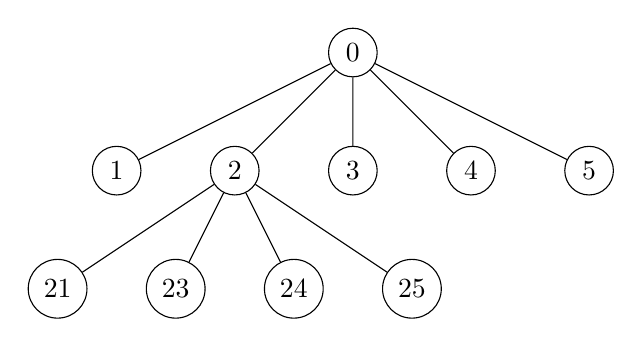
\begin{tikzpicture}[every node/.style={draw,circle}]
  \node (0) {0}
  child {node(1) {1}}
  child {node(2) {2}
    child {node(21) {21}}
    child {node(23) {23}}
    child {node(24) {24}}
    child {node(25) {25}}
  }
  child {node(3) {3}}
  child {node(4) {4}}
  child {node(5) {5}};
\end{tikzpicture}

The number of keys each node needs to keep will be increased
exponentially as $n - k$ becomes big. Up to $(7,10)$ threshold seems
practical.

\subsubsection*{DSA, ECDSA}
BFTKV implements a DSS threshold scheme introduced by Gennaro et
al.\ \cite{Gennaro}.
Since the scheme has a restriction such that $n \geq 2t$ in the $(t,
n)$-threshold scheme, we no longer be able to use the quorum threshold
for $(t, n)$. But, we follow the protocols between the client and a
quorum, i.e., the client sends a signing request to a quorum
(multicast the message to all quorum members), then collect the
responses. Our signing protocol consists of three phases:
\begin{enumerate}
\item Collect joint shared secrets generated by each quorum member
\item Distribute the secrets to the quorum and calculate
  $r=g^{k^{-1}} \bmod p \bmod q$ where $k$ is the
  joint Shamir's shared secret (i.e., $k = \sum k_i$)
\item Distribute r to the quorum and calculate $s=k(m+xr) \bmod q$
  from each $s_i=k_i(m+x_ir) \bmod q$ returned from each quorum member
\end{enumerate}
